\documentclass[10pt,a4paper]{article}
\usepackage[latin1]{inputenc}
\usepackage{amsmath}
\usepackage{amsfonts}
\usepackage{amssymb}
\usepackage{graphicx}
\usepackage{url}
\usepackage{color}
\usepackage{listings}

\author{Amar, Meghana, Giuseppe, Rapha\"el}
\title{Spotting and Disambiguating Events from Social Live Streams}
%\title{EventSpotter: Spotting entities that talk about events}

\begin{document}
\maketitle
\section{Introduction}
Social event sharing websites such as last.fm, Eventful, Eventbrite, and Facebook contain the most precise and up to date information related to scheduled or planned events. 
%The dynamic nature of these platforms allows to have a continuos stream. 
Generally an event is characterized by the surface form (title), and additional features such as category, location, time, and agents (who perform the event). Spotting an event therefore means traversing a multi-dimensional space, labelled by a clear ambiguos definition given by the event name. 
In the literature different approaches have narrowed down the event extraction task in an entity extraction one. But the complexity of the extraction task increases manifold in the event domain. The biggest challenge of this task is to obtain a clear unambiguous definition of an event title. This is because there is a lack of uniform rule based nomenclature with respect to events. 
%{\color{red}{G:need to cut off the many examples, which are verbose}}\newline
For instance, it is common practice for musical events to be named after the artists who are performing at the event. 
%Here, the event title is ``Beth Jeans Houghton'' which is also the name of the performing artist. 
This brings in a word sense disambiguation problem, where the onus is on comprehending whether the spot refers to the artist or to the event. The next level of complexity is introduced when an event title is created as an amalgamation of the artist names, band names, event venue and at times even the date, using special characters. %Here, ``Stay Sharp Album Release Party: Higher Hands + Grilled Lincolns + Pressing Strings'' is an event title as per the information uploaded on the event sharing website ``eventful''. 
In essence this means any stripping or stop-wording of input text, which would have otherwise been a natural choice for a preprocessing step in any information extraction problem, is completely out of question. This also means the length of an event title may range from just one word to a phrase with many words and punctuations. Further, at times the boundaries of creative license are stretched to the point where events are named with words that don't even exist in the language vocabulary. 
%Here, ``Pocktoberfest'' is an yearly event which takes place at the ``Pocklington arts center''. But the word ``Pocktoberfest'' does not exist in the English language. 
%If all events followed a standard naming scheme, our task which now seems herculean, would have been average, at best. 
The live nature of the event detection makes further complex the extraction process, that results in a partial lack of benchmark from which to start a canonical natural language chain. In this work we explore the plausibility of using a mixture of various information extraction and semantic web techniques to event detection and demonstrate that it is possible to obtain an increase in recall even with a linear combination of linguistic and knowledge based approaches grounded on a live stream of social event data to spot and disambiguate event entities in plain text.

\section{Approach}
The live social event data stream is pivotal for our approach. We use the EventMedia dataset~\cite{krouf2012}, which offers an always updated window on the events which are spread across different social platforms. We incrementaly compute snapshots of the dataset and we build on top of it our event lexicon indexer, which acts as an event knowledge base, \textit{de-facto} bulk of the proposed work. Our approach is then composed of the following stages: \textit{i)} preprocessing, \textit{ii)} candidate selection and \textit{iii)} disambiguation. \textit{i)} is orthogonally applied for normalizing the EventMedia events and for every textual input, the data is first tokenized, then converted to the CoNLL IOB format. To aid the second stage, we added five additional features to the dataset: capitalization information (initial capital, allcaps), prefix (first three letters of the token), suffix (last three letters of the token), digit.
\textit{ii)} checks for a case-insensitive match with the tokenized version of the indexer of events. The reason for performing such a case insensitive match is to ensure that we encompass all candidate event names, without losing any because of an insignificant case-sensitive mismatch. We call this type of mismatch insignificant because of the fact that since we consider unstructured input text, it is quite possible that event names may not be highlighted consistently in the same manner of case. The aim is to start with the largest set of candidate events and gradually limit the set to confirmed events by disambiguation. 
\textit{iii)} ascertains the validity of each entry in the candidate list with the help of metadata stored in the EventMedia dataset. 
%The proven hypothesis is that for a knowledge based approach to event detection, to identify only those events which are reasonably described in the input text. We consider an event as reasonably described if and only if there is a mention of : at least one of the agents (performing artists) or  the location (event venue) in the input text. In other words, this means that many events may go undetected in cases where the agent or the location string is not present in the input text. Though this would affect the recall of the system, we felt that it would be a trade-off worth making. This is primarily because, a large number of events are titled with commonly used words in a language. This means that any strategy that adopts an approach that is less restrictive would end up with a many false positive results. 
%As mentioned earlier, we recognize that basing our approach solely on the first hypothesis, will not allow us to achieve a near-exhaustive detection of event entities in the text. Hence, we intend to deal with these false negatives by employing a linguistic approach in the second pass to detect those events which are not reasonably described in the input text. 
For each candidate event it looks up the EventMedia normalized dataset to get the named of agents who had performed at that event. It then tries to spot these  agent tokens in the input text using the naive spotter described in the candidate selection stage. If at least one agent is found in the input text then the candidate spot is considered as a valid event and added to the list of detected events. Also for each validated candidate spot it computes a cosine similarity measure between the surroundings of the spot and the event description. The event description contains other key information such as location, sentimental expressions such as ``thrilling'', ``exciting'' and ``mindblowing'' ; entry fee ; domain specific terms such as ``rock'', ``music'', ``concert''; some historical background about the artists, events and so on. These are aspects which are unique to each event and there is a mention of some or all of these attributes in each event description. This way we manage to match various miscellaneous attributes of an event which can, generally not be categorized into fields such as agents, location etc. We empirically defined the surroundings to be the current, previous and next sentences from the spot. This cosine similarity measure is considered as the confidence score for each valid spot. The disambiguation stage yields a list of detected event titles and their respective confidence scores.

{\color{red}{A+M: redo the figure, remove upcoming logo and add Eventbrite, Facebook logos}}
Figure~\ref{fig:architecture} shows the architectural diagram of the proposed approach called EventSpotter. 

%\begin{lstlisting}
%Input : unstructured text 
%Output : disambiguated musical events
%
%# Start the preprocessing by tokenizing input text
%tokens = tokenize(input)
%
%sentences = sentensize(input)
%
%#Candidate Selection
%candidates = doSpotting(input, tokens, entries)
%# entries is a list of tokens obtained by tokenizing the list of event titles file
%# candidates are case insensitive matches of tokens with entries
%
%#Disambiguation
%for each candidate in candidates
% if candidate doesn''t start with capital letter and first char is not a digit
%  then continue to next candidate
% end if
%
% List<String> agents = geatagents(eventId)
% Set<FeatureStructure> foundAgentToks = doSpotting(input, tokens, agents)	
%	
% if atleast one agent is found in the input text  
%  then get surroundings to compute confidence score		
%  Surround = getSurrounding(sentences,candidate);
%  #If candidate is in the first line of input text, current and next line is surrounding.
%  #If candidate is in the middle of input text, previous, current and next line is surrounding.
%  #If candidate is in the last line of input text, current and previous line is surrounding.
%
%  confidence = cosine similarity.run(Surround,event description)
%	 
%  confirm candidate as an event and add to FeatureStructure.
% endif	
%endfor
%#Post processing
% Add <EVENT> tags to input text 
% Display annotated input text 
% Display spotted events with confidence score in JSON format
%\end{lstlisting}

\begin{figure}
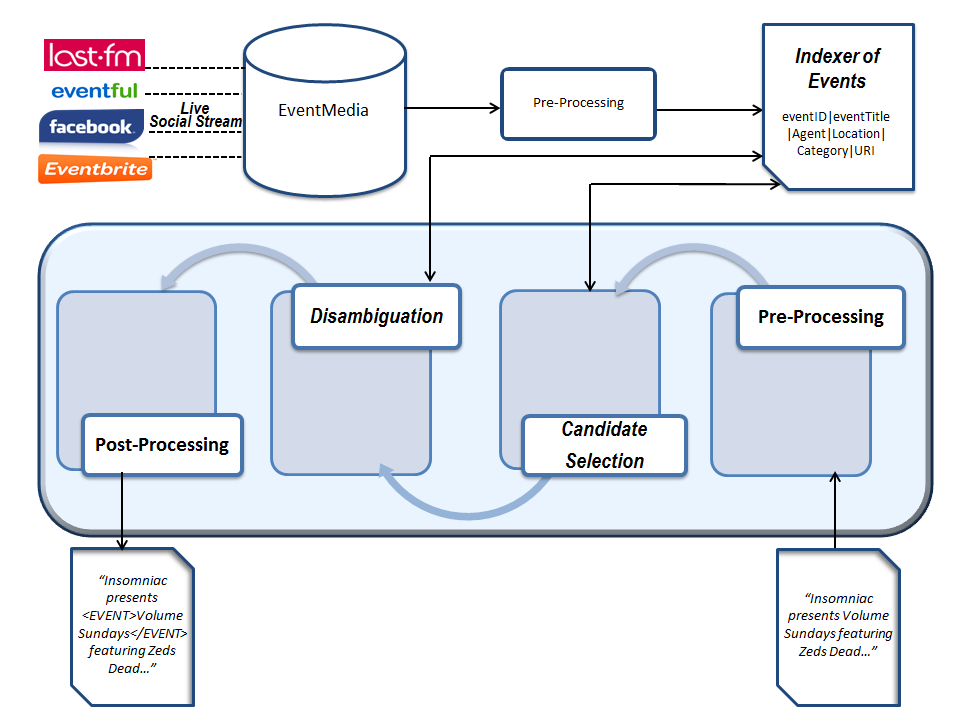
\includegraphics [width=13cm,height=6cm]{architecture}
\caption{EventSpotter system}
\label{fig:architecture}
\end{figure}


\section{Benchmark}
Even though one of the strengths of the EventSpotter approach was to rely on a continuously updated, dynamic, live event knowledge base. We used a static benchmark to perform a canonical evaluation to compare this approach with the state of the art systems. We created an in-house benchmark, which was supervised by 4 human raters who achieved a good agreement score. In this benchmark we assessed both NER and NEL tasks.

The EventSpotter project makes use of a snapshot of the EventMedia to detect all musical events that occurred in 2012. Thus, it is obvious that the test corpus must contain only events that occurred in this year. To the best of our knowledge no such corpus existed and so we were faced with the ardous task of creating one. However, instead of starting from scratch we decided to use event descriptions from the EventMedia dataset and annotate them. Since event descriptions in the dataset were essentially texts uploaded by multiple users onto various event sharing sites, using them as test corpora would help simulate a real world test scenario. But the EventMedia dataset contains close to 65,000 entries and it was neither feasible nor necessary for the evaluation stage of our project to use all these event descriptions. Instead we selected 100 event descriptions at random, such that this test sample represented the entire EventMedia dataset in an apt and unbiased manner. Before annotating these documents we preprocessed them to ensure that all HTML tags and URLs were removed so as to facilitate the creation of a clean golden dataset. We further reduced the size of the corpus to 60 documents by selecting only those that were in written in English. These documents can be found at \url{https://github.com/amark-india/eventspotter/tree/master/data}. 

For experimental purposes, we followed 2 types of annotation: synthetic annotation and manual annotation.
In the case of synthetic annotation, we carried out a straightforward string comparison between the input text and all event titles in the EventMedia dataset. Every match was considered as a valid spot and was annotated as an event. Adopting this synthetic approach was not only aided in quickly establishing a base to assess the performance of the EventSpotter. But also, came in handy during the training phase of the Stanford CRF classifier. We will see during the presentation of the results that the Stanford CRF classifier performed quite differently with synthetically annotated training data when compared to manually annotated training data. Finally, we realised by observation, that some aspects of the synthetic annotation approach could be applied during the manual annotation process.

As we performed manual annotation, we realised that there was an inherent ambiguity in event titles. We found it extremely difficult, at times, to distinguish between event titles and artist names. Mainly because events were often titled as a mash up of the artist names, venue and sometimes the date of occurrence. Due to this ambiguity many event titles were not annotated despite strict adherence to the annotation rules. Thus, it made sense to not rely solely on the annotators'' knowledge, but in fact, partially adopt the synthetic annotation approach in order to generate a more robust golden dataset. The manual annotation was broken down into two passes. In the first pass, an unbiased, rule based manual annotation was performed. In the second pass, the human annotators were given the list of event titles that were being described in the documents. With this posteriori knowledge the human annotators were able to annotate event occurrences which would have otherwise gone unnoticed. As human annotators, we leveraged the context of the spot to perform word sense disambiguation. We refrained from annotating those spots where in the event title string was not used to directly refer to the event itself. In the phrase ``Carrie Underwood announces her North American tour Blown Away'', ``Carrie Underwood'' referred to the artist, not the event title and hence was not annotated (see example 8.1). But in another instance, ``Carrie Underwood comes to town this Monday.'' since the annotator knew that Carrie Underwood was the event title and since this string was being used to refer to an event in this context, the spot was annotated as an event (see example 8.2). We observed that this hybrid approach towards manual annotation was effective in improving the golden dataset and this was corroborated by the improvement in performance results as presented in the following section.

{\color{red}{A+M:Details of the dataset (see how to explain the differences between synthetic and manual.}}

{\color{red}{A+M:create a table with the stats of the dataset, i.e. number of token etc. etc.}}

{\color{red}{A+M:point to the dataset (GitHub URI).}}

\section{Experiments and Results}
We performed 10-fold cross validation and found that the EventSpotter performed better than the Stanford CRF in terms of recall and F-measure.

As baselines OpenCalais (as off-the-shelf solution) and Stanford NER, properly trained with the data of the training set. A long survey on off-the-shelf systems able to detect events resulted to depict an extremely specific domain, where systems are tailored for performing reasonably well on specific data. This consideration is further proven by the results achieved and it explain why OpenCalais is not able to detect musical events. For this reason, we omit to report the OpenCalais results.

Results are computed using the conlleval script\footnote{\url{http://www.cnts.ua.ac.be/conll2002/ner/bin/conlleval.txt}} and plotted using R. It obtained a score of 89.26\% for recall and 72.73\% for F-measure, over the scores of 4.27\% and 8\% respectively of the Stanford NER trained with synthetic annotation and 54.70\% and 60.95\% respectively when trained with manual annotation. To highlight once again, these set of tests on the synthetically annotated golden dataset were carried out merely to give ourselves an idea about the EventSpotter's performance. Opencalais did not identify any musical event entities at all. Opencalais detects events from various categories which does not include musical festival or concert. Since it does come close with the category ``musical bands'' we thought it would be interesting to note how many events it would detect.
\begin{table}[ht]
\centering % used for centering table
\begin{tabular}{c c c c} % centered columns (4 columns)
\hline\hline %inserts double horizontal lines
Approach & Precision & Recall & F-Measure \\ [0.5ex] % inserts table
%heading
\hline % inserts single horizontal line
EventSpotter & 61.36\% & \bf 89.26\% \bf & \bf 72.73\% \bf \\ % inserting body of the table
Stanford trained on synthetic data & 62.5\% & 4.27\% & 8\%\\
Stanford trained on manual data & \bf 68.82 \bf \% & 54.70\% & 60.95\% \\
Opencalais & 0\% & 0\% & 0\% \\
\hline %inserts single line
\end{tabular}
\caption{Tests Performed with Synthetically Annotated Golden Dataset with 122 valid event annotations} % title of Table
\label{table:nonlin} % is used to refer this table in the text
\end{table}

The second set of tests run were run on the manually annotated golden dataset which contained 115 valid event annotations. Again the EventSpotter's performance out-shined that of the Stanford CRF in terms of recall and F-measure. It obtained a score of 68.14\% for recall and 43.14\% for F-measure, over the scores of 54.87\% and 56.88\% respectively of the Stanford CRF trained with synthetic annotation and 11.5\% and 18.71\% respectively when trained with manual annotation. Again, Opencalais did not identify any musical event entities at all. We also tested a linear combination of EventSpotter and Stanford CRF trained on synthetically annotated data, with Stanford CRF acting as a gazetteer to EventSpotter. Though there wasn't a stark improvement, the recall score did increase slightly to 70.8\%.
\begin{table}
\centering % used for centering table
\begin{tabular}{c c c c} % centered columns (4 columns)
\hline\hline %inserts double horizontal lines
Approach & Precision & Recall & F-Measure \\ [0.5ex] % inserts table
%heading
\hline % inserts single horizontal line
EventSpotter & 31.56\% & \bf 68.14\% \bf & 43.14\% \\
Stanford trained on synthetic data & \bf 59.05\% \bf & 54.87\% & 56.88\%\\
Stanford trained on manual data & 50\% & 11.5\% & 18.71\% \\
Stanford Gazetteer to EventSpotter & 31.25\% & \bf 70.8\% \bf & 43.36\% \\
Opencalais & no events & no events & no events \\
\hline %inserts single line
\end{tabular}
\caption{Tests Performed with Manually Annotated Golden Dataset with 115 valid event annotations} % title of Table
\label{table:nonlin} % is used to refer this table in the text
\end{table}

\section{Discussion and outlook}
Thus by relying on a live social data stream we demonstrate that our approach can overcome the static nature of other rigid rule based approaches such as Conditional Random Field classifiers. In our approach we first use the social event data to identify candidate events, then disambiguate these candidate spots using event attributes such as artists, venue, date, event description and category. and assign a confidence score based on a cosine similarity with the event descriptions from EventMedia. 

{\color{red}{G:Outlook.}}

The experiments detailed in this paper are reproducible and the source code is available at \url{https://github.com/amark-india/eventspotter}. 


\bibliographystyle{plain}
\bibliography{eventspotter}
\end{document}